%
% teil1.tex -- Beispiel-File für das Paper
%
% (c) 2020 Prof Dr Andreas Müller, Hochschule Rapperswil
%
% !TEX root = ../../buch.tex
% !TEX encoding = UTF-8
%
\section{Crash Kurs Erd- und Raketen-Physik
\label{leo:section:physik}}
\rhead{Crash Kurs Erd- und Raketen-Physik}
Die Dynamik des Fahrzeugs während des Aufstiegs in den Low Earth Orbit wird durch eine Reihe von Differentialgleichungen beschrieben, die das Verhalten der Zustandsvariablen über die Zeit charakterisieren. 
Diese Gleichungen sind ein zentraler Bestandteil des Variationsproblems und ermöglichen die Berechnung der optimalen Steuerungstrajektorie. Diese werden in hier nun kurz beschrieben.
Die Grundlagen sind dem Buch Astronautics von Ulrich Walter \cite{leo:astronautics} entnommen.


\subsection{Zustands- und Steuervariablen\label{leo:section:variabeln}}
\rhead{Zustands- und Steuervariablen}
In diesem Kapitel wird die Berechnung einer möglichst Effizienten Flugbahn von der Erde in den LEO (Low Earth Orbit) hergeleitet. 
Die Rakete startet senkrecht auf Meereshöhe aus dem Stillstand. 
Sie muss die Höhe für den LEO erreichen, waagrecht sein und eine bestimmte Geschwindigkeit haben um im LEO zu bleiben. 
Die folgenden Zustands- und Steuervariablen beschreiben die Rakete werden diesem Flug.
In Fig.\,\ref{fig:leo:forces} sind diese veranschaulicht.

\begin{itemize}
	\item $\alpha$: Steuerungswinkel  zur momentanen Raketenrichtung
	\item $\gamma$: Winkel zum lokalen Horizont
	\item $v$: Maximal Geschwindigkeit der Rakete
	\item $v_f$: Momentane Geschwindigkeit der Rakete
	\item $H$: Zu erreichende Höhe
	\item $h$: Momentane Raketehöhe zur Startpunkt
	\item $m_0$: Treibstoff Masse beim Start der Rakete
	\item $m_f$: Masse der Rakete ohne Treibstoff
	\item $t_f$: Zeit bis Rakete im Orbit ist
	\item $m$: Gesamt Gewicht der Rakete
\end{itemize}

\begin{figure}
	\centering
	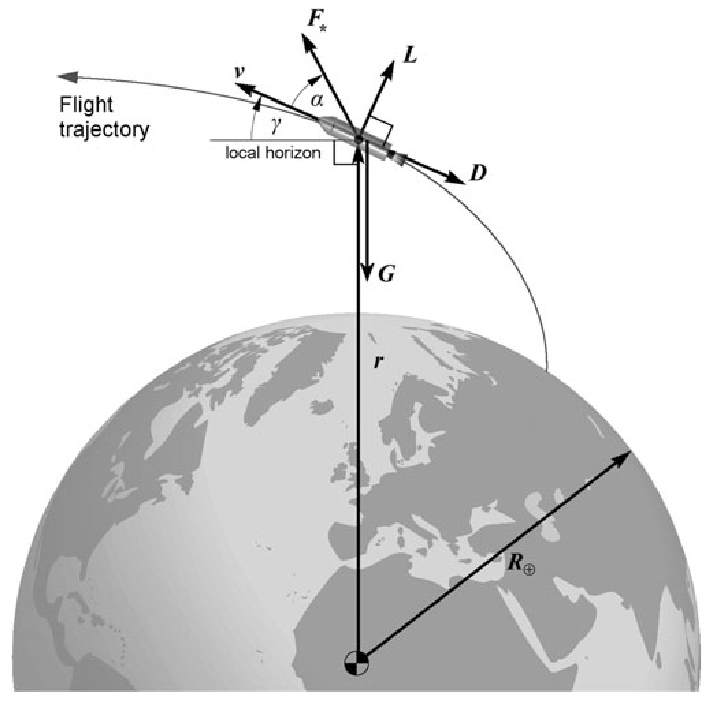
\includegraphics[width=0.5\linewidth]{papers/leo/Grafiken/forces.png}
	\caption{Zustands- und Steuervariablen veranschaulicht entnommen von \cite{leo:astronautics}.}
	\label{fig:leo:forces}
\end{figure}


\subsection{Raketendynamik}
\todo{Bewegungsgleichungen ausführen}
\begin{itemize}
	\item DGL zum Beschreiben der Dynamik \[\mathbf{\dot{x}} = (\dot{\gamma},\dot{v},\dot{x},\dot{h})\]
\end{itemize}
\begin{align*}
	\dot{v} &= \frac{F_*}{m} \cos \alpha - \frac{D}{m} - g \sin \gamma \\
	\dot{\gamma} &= \frac{1}{v}\left( \frac{F_*}{m} \sin \alpha + \frac{L}{m} - \left(g - \frac{v^2}{r}\right) \cos \gamma \right)\\
	\dot{h} &= v \sin \gamma \\
	\dot{x} &= v \cos \gamma        
\end{align*}


\subsection{Antrieb}
Die Form einer Rakete beeinflusst die Aerodynamik und den Treibstoffverbrauch. 
Der Treibstoffverbrauch wiederum hängt von der Art der Triebwerke und des Treibstoffs ab.
Die Rakete selbst soll leicht sein, muss aber enormen Kräften standhalten.
All diese Faktoren fließen in die klassische Raketengrundgleichung ein
\begin{equation}
	v_f = v_* \ln \left(\frac{m_0}{m_f}\right)
	\label{leo:raketengleichung}
\end{equation}
ein.
$v_f$ ist die maximale Geschwindigkeit, die eine bestimmte Rakete erreichen kann.
Dabei ist $m_0$ die Anfangsmasse des Treibstoffs und $m_f$ die Masse der Rakete. 
$v_*$ ist ist die effektive Abgasgeschwindigkeit von einem Triebwerk.
Die hängt vom Treibstoff und dem Triebwerk ab.


Die Steuerung der Rakete bedeutet einen Verlust, da der Luftwiderstand durch eine größere Angriffsfläche erhöht wird und ein Teil der Treibstoffenergie zur Steuerung der Rakete verwendet wird. Dieser Verlust kann in einer Geschwindigkeit von
\begin{equation}
	v_s = 2F_* \int_0^{t_f} \frac{\sin^2\left(\frac{\alpha}{2}\right)}{m} \, dt
	\label{leo:raketenluftwiderstand}
\end{equation}
ausgedrückt werden.
$F_*$ ist der Gesamtschub welcher von $v_*$ hergeleitet werden kann.


\subsection{Schwerkraft}
Die Schwerkraft ist die größte Kraft, die eine Rakete überwinden muss, um in den Weltraum zu gelangen. 
Sie nimmt mit zunehmender Höhe ab. 
Um eine stabile Umlaufbahn zu erreichen, muss die Rakete schneller um die Erde fallen, als sie auf die Erde fällt. 
Die Geschwindigkeit der Rakete muss also größer sein als die Fallgeschwindigkeit. 
Mit 
\begin{equation}
	v_g =\int_0^{t} g \sin \left(\gamma\right) \, dt
	\label{leo:schwerkraftswiderstand}
\end{equation}
kann berechnet werden, wie stark die Schwerkraft die Rakete abbremst. 
Dabei spielt es eine Rolle, ob die Rakete den Schub direkt gegen die Schwerkraft ausübt oder nicht. 
Dies fließt mit $\gamma$ in die Gleichung ein.

\subsection{Atmosphäre}
% Der Luftwiderstand $D(t)$ wirkt entgegen der Bewegungsrichtung des Fahrzeugs und ist abhängig von der Geschwindigkeit sowie der Luftdichte. 
% Die Luftdichte $\rho(y)$ nimmt linear mit der Höhe $y$ ab, was durch die Gleichung $\rho(y) = \rho_0 (1 - \alpha y)$ dargestellt wird, wobei $\rho_0$ die Dichte auf Meereshöhe und $\alpha$ die Abnahmerate der Dichte mit der Höhe ist.

% Der Luftwiderstand wird durch
% \[
% D(t) = \frac{1}{2} \rho(y(t)) C_d A v^2(t)
% \]
% wobei $C_d$ der Luftwiderstandsbeiwert, $A$ die Querschnittsfläche des Fahrzeugs und $v(t) = \sqrt{v_x^2(t) + v_y^2(t)}$ die Gesamtgeschwindigkeit des Fahrzeugs ist. 
% Der Luftwiderstand wirkt sowohl auf die horizontale als auch auf die vertikale Geschwindigkeitskomponente, basierend auf deren Anteilen an der Gesamtgeschwindigkeit.
Der Luftwiderstand $D(t)$ wirkt entgegen der Bewegungsrichtung des Fahrzeugs und ist abhängig von der Geschwindigkeit sowie der Luftdichte. 
Die Luftdichte $\rho(y)$ nimmt mit der Höhe $y$ ab.
Sie ist dabei aber nicht nur Abhängig von der Höhe sondern auch vom Wetter, der Temperatur, der Sonnenaktivität und vielem mehr.
Oft werden deshalb Modelle als Annäherung gebraucht.
Der Luftwiderstand wird durch
\begin{equation}
	D(t) = \frac{1}{2} \rho(y(t)) C_d A v^2(t)
\end{equation}
berechnet.
$C_d$ ist der Luftwiderstand, $A$ die Querschnittsfläche des Fahrzeugs und $v(t)$ die Gesamtgeschwindigkeit des Fahrzeugs ist. 
Der Luftwiderstand wirkt basierend auf deren Anteilen an der Gesamtgeschwindigkeit.

Dieser Strömungsverlust kann in
\begin{equation}
	v_l = \frac{1}{H} \int_0^{t_f} k_Dv^2 e^{-\frac{h}{H}} \, dt
	\label{leo:strömungsverlust}
\end{equation}
ausgedrückt werden, welcher den Verlust in einer Geschwindigkeit berechnet.
Dieser Strömungsverlust ist natürlich noch abhängig von der Geschwindigkeit und der Höhe.
Der Luftwiderstand wird vereinfacht zu einer konstanten $k_D$. 


